\documentclass[12pt,a4paper]{report}
\usepackage[brazil]{babel}
\usepackage[]{algorithm}
\usepackage[]{algorithmic}
\usepackage[style=numeric,backend=biber]{biblatex}
\usepackage[utf8]{inputenc}
\usepackage{kpfonts}
\usepackage[T1]{fontenc}
\usepackage{wrapfig}
\usepackage{graphicx}
\usepackage{enumerate}
\usepackage{subcaption}
\usepackage{float}
\usepackage{caption}
\usepackage{listings}
\usepackage{lipsum}
\usepackage{amsthm}
\usepackage{amssymb}
\usepackage{bm}
\usepackage{color}
\usepackage{afterpage}
\usepackage[inline]{enumitem}
\usepackage{pdflscape}
\usepackage{listingsutf8}
\usepackage{siunitx}
\usepackage{bashful}

\graphicspath{ {./images/} }

\lstset{frame=tb,
  aboveskip=2mm,
  belowskip=2mm,
  showstringspaces=false,
  columns=flexible,
  basicstyle=\footnotesize,,
  numbers=left,
  numbersep=5pt,
  stepnumber=1,
  breaklines=true,
  keepspaces=true,
  breakatwhitespace=true,
  showtabs=false,  
  tabsize=2
}

% Definindo estilo para os códigos
\definecolor{mGreen}{rgb}{0,0.6,0}
\definecolor{mGray}{rgb}{0.5,0.5,0.5}
\definecolor{mPurple}{rgb}{0.58,0,0.82}
\definecolor{dkgreen}{rgb}{0,0.6,0}
\definecolor{backgroundColour}{rgb}{0.97,0.97,0.97}

\lstset{basicstyle=\ttfamily,
    backgroundcolor=\color{backgroundColour},   
    commentstyle=\color{mGreen},
    keywordstyle=\color{magenta},
    numberstyle=\tiny\color{mGray},
    commentstyle=\color{dkgreen},
    stringstyle=\color{mPurple},
    basicstyle=\footnotesize,
    breakatwhitespace=false\textbf{,}         
    breaklines=true,                 
    captionpos=b,                    
    keepspaces=true,                 
    numbers=left,                    
    numbersep=5pt,                  
    showspaces=false,                
    showstringspaces=false,
    showtabs=false,                  
    tabsize=2,
    language=bash
}

\lstdefinestyle{BStyle}{
    backgroundcolor=\color{backgroundColour},  
    showstringspaces=false,
    numbers=none,
    language=bash
}

\pagenumbering{arabic}
\renewcommand{\thesection}{\arabic{section}}

\bibliography{ref}
\renewcommand{\contentsname}{Sumário}{\thispagestyle{empty}}
\renewcommand{\baselinestretch}{1.5} 

\begin{document}

\begin{titlepage}
    \begin{center}
        \vspace*{1cm}
        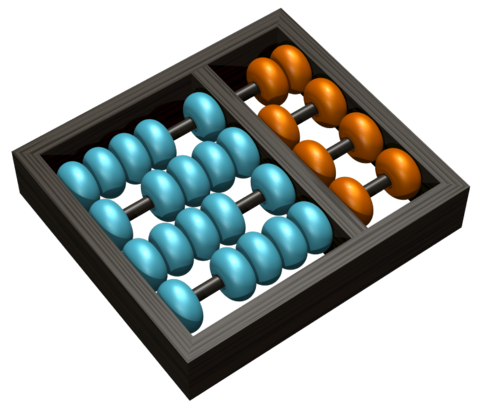
\includegraphics[width=0.25\textwidth]{Logo}\\
        \vspace{1.5cm}
        \Huge
    	\textbf{MC833 Relatório 3 \\
        Cliente e servidor TCP} \\
        \vspace{1.5cm}
        \Large
        \textbf{Aluno}: Fábio Camargo Ricci\\
        \textbf{RA}: 170781\\
        \vspace{1.2cm}
    	\Large 
    	Instituto de Computação\\
    	Universidade Estadual de Campinas\\
    	\vspace{1.5cm}
        Campinas, 19 de Setembro de 2021.
    \end{center}
\end{titlepage}
\tableofcontents
\clearpage

\newcommand{\shellcmd}[1]{\texttt{\footnotesize\# #1}}%estilizando citação de comandos do shell

\section{Questões}

\begin{enumerate}
    \item Analise os códigos dos programas cliente.c e servidor.c e identifique as funções usadas para comunicação via socket. Procure nas páginas de manual do Linux, a descrição das funções que estão relacionadas ao uso de sockets. Procure também nos códigos a natureza dos parâmetros que cada programa deve receber, se for o caso.
    
    \item Compile e execute os programas cliente.c e servidor.c em uma mesma máquina. Houve algum erro? Em caso afirmativo, qual a sua causa? Se necessário, modifique os programas de forma que este erro seja corrigido e informe quais modificações foram realizadas. (Insira uma figura mostrando que o seu código executou sem erros)
    
    \item Altere o código do servidor para que seja automatizado a escolha da porta e utilize sempre o IP da máquina que está sendo executado.
    
    \item Liste as chamadas de sistema necessárias para um servidor escutar conexões futuras. Justifique.
    
    \item Modifique o programa cliente.c para que ele obtenha as informações do socket local (\#IP, \#porta local) através da função getsockname().
    
    \item Modifique o programa servidor.c para que este obtenha as informações do socket remoto do cliente (\#IP remoto, \#porta remota), utilizando a função getpeername(). Imprima esses valores na saída padrão.
    
    \item É possível usar o programa telnet no lugar do binário do cliente.c? Justifique e comprove sua resposta.
\end{enumerate}

\section{Respostas}

\begin{enumerate}
   \item Funções usadas para comunicação via socket:
   \begin{enumerate}
        \item \textbf{socket}(int \textbf{domain}, int \textbf{type}, int \textbf{protocol}): Cria um  endpoint de comunicação e retorna um file descriptor que referencia o mesmo.
       \begin{enumerate}
            \item \textbf{domain}: Refere-se ao domínio de comunicação (a família de protocolos que será utilizada para comunicação).
            
            \item \textbf{type}: Especifica as semânticas de comunicação.
            
            \item \textbf{protocol}: Indica qual protocolo de comunicação será utilizado
        \end{enumerate}
        
        \item \textbf{bind}(int \textbf{sockfd}, const struct sockaddr *\textbf{addr}, socklen\_t \textbf{addrlen}): Relaciona um nome a um socket. Quando um socket é criado, o mesmo existe em uma família de endereços mas não possui um endereço atrelado. O método \textbf{bind()} atrela o endereço especificado por \textbf{addr} ao socket \textbf{sockfd}. \textbf{addrlen} indica o tamanho, em bytes, da estrutura apontada por \textbf{addr}.
        
        \item \textbf{listen}(int \textbf{sockfd}, int \textbf{backlog}): Espera por conexões em um socket. O método marca o socket indicado por \textbf{sockfd} como um socket passivo, esperando conexões através de \textbf{accept()}. \textbf{backlog} indica quantas conexões pendentes para o determinado socket podem existir.
        
        \item \textbf{accept}(int \textbf{sockfd}, struct sockaddr *restrict \textbf{addr}, socklen\_t *restrict \textbf{addrlen}): Aceita uma conexão em um socket. \textbf{sockfd} se refere a um socket passivo que está escutando conexões, que foi criado com \textbf{socket()}, atrelado a um endereço com \textbf{bind()} e estava esperando por conxões com \textbf{listen()}. \textbf{addr} é um ponteiro para um estrutura do tipo \textbf{sockaddr}, que é populada com o endereço do socket sendo conectado (par). \textbf{addrlen} é o tamanho, em bytes da estrutura \textbf{addr}. Esse método cria um novo socket conectado (baseado no socket passivo criado anteriormente) que estará atrelado à nova conexão e servirá como meio de comunicação.
        
        \item \textbf{connect}(int \textbf{sockfd}, const struct sockaddr *\textbf{addr}, socklen\_t \textbf{addrlen}): Inicia uma conexão com um socket. Esse método conecta o socket descrito por \textbf{sockfd} ao endereço especificado por \textbf{addr}.
   \end{enumerate}
   
   \item Não houve nenhum erro ao executar o cliente ou servidor. Compilou-se os programas com os comandos:\\
   \textit{gcc -o servidor servidor.c -Wall}\\
   \textit{gcc -o cliente cliente.c -Wall}
   
   As saídas obtidas foram:\\\\
   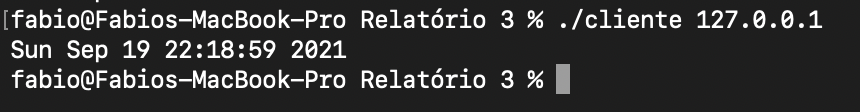
\includegraphics[width=13cm]{images/cliente.png}\\\\
   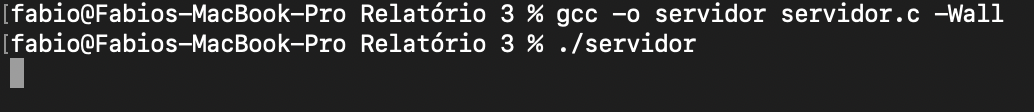
\includegraphics[width=13cm]{images/servidor.png}
   
   \item Atribuindo a constante INADDR\_ANY ao endereço do socket servidor (\textbf{servaddr.sin\_addr.s\_addr = htonl(INADDR\_ANY)}), o mesmo passa a aceitar conexões em todos os endereços IPs disponíveis no host (após a chamada do método \textbf{bind()})
   \\
   Para automatizar a escolha da porta, atribuiu-se o valor de \textbf{servaddr.sin\_port = 0}, de modo que fica a cargo do sistema escolher uma porta disponível.
   \\
   \\
   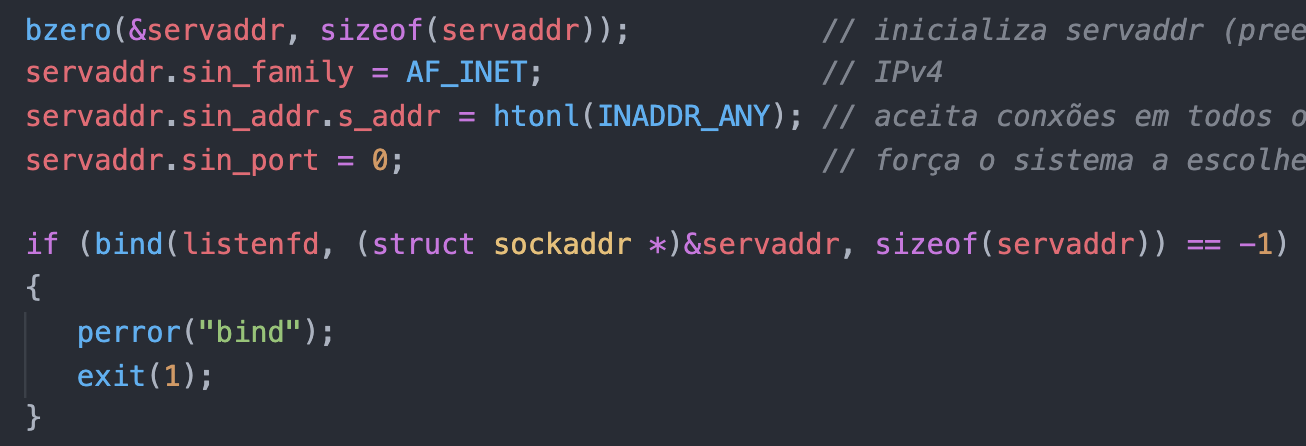
\includegraphics[width=13cm]{images/ex3.png}

 
   \item Para um servidor escutar conexões futuras, são necessárias quatro chamadas de sistema (descritas em detalhes na questão 1):
    \begin{enumerate}
        \item \textbf{socket}(int \textbf{domain}, int \textbf{type}, int \textbf{protocol}): Cria o socket que servirá como meio para a comunição.
        
        \item \textbf{bind}(int \textbf{sockfd}, const struct sockaddr *\textbf{addr}, socklen\_t \textbf{addrlen}): Atrela o socket acriado anteriormente a um endereço.

        \item \textbf{listen}(int \textbf{sockfd}, int \textbf{backlog}): Espera por conexões futuras em um socket, marcando o mesmo como um socket passivo. Possui uma fila de conexões pendentes com tamanho de \textbf{backlog}.
        
        \item \textbf{accept}(int \textbf{sockfd}, struct sockaddr *restrict \textbf{addr}, socklen\_t *restrict \textbf{addrlen}): Aceita uma nova conexão no socket passivo descrito, criando um novo socket conectado que estará atrelado à nova conexão.
    \end{enumerate}
    
    \item A função \textbf{getsockname()} recupera as informações do endereço do socket local (atribuído ao chamar \textbf{bind()} anteriormente). Com isso, utilizou-se a função \textbf{inet\_ntop()} para obtermos a representação em string IPv4 do endereço obtido.
    \\\\ 
    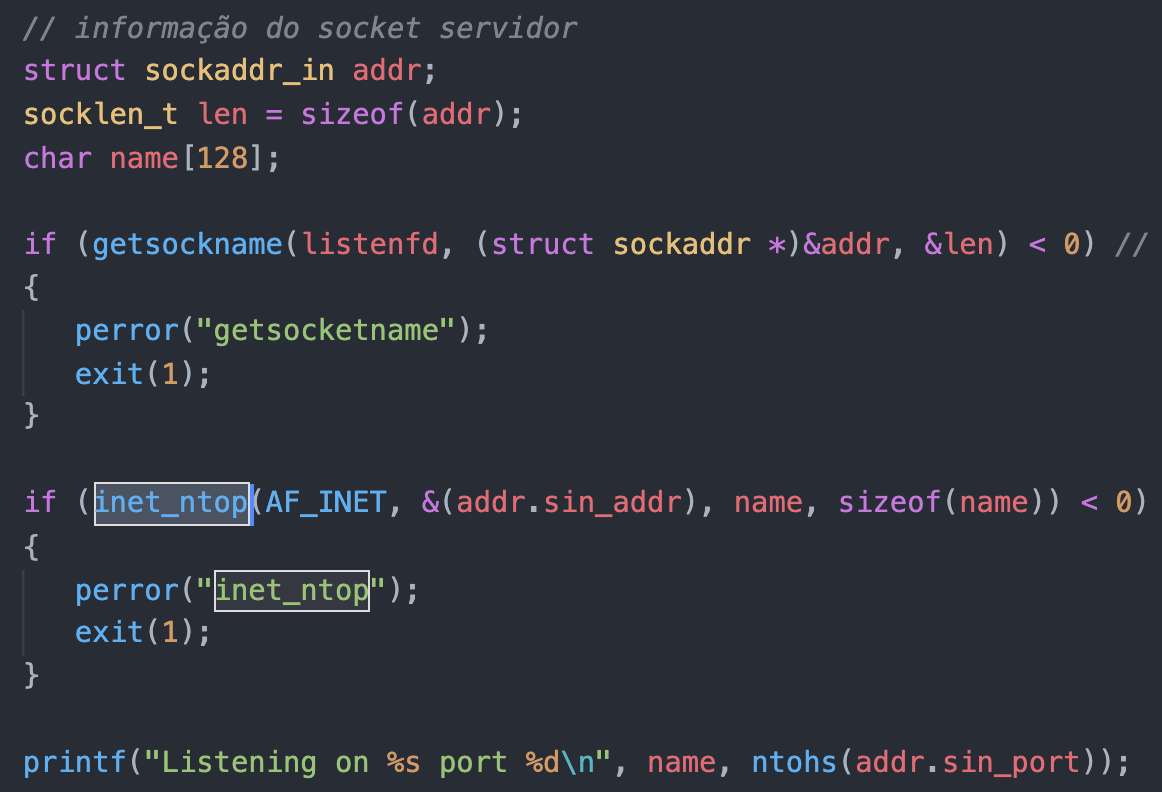
\includegraphics[width=13cm]{images/ex6-servidor.png}
    \\
    No cliente, alterou-se o código para aceitar o endereço IP e a porta que o servidor está escutando (previamente so aceitava o endereço IP, com a porta fixa). 
    \\\\
    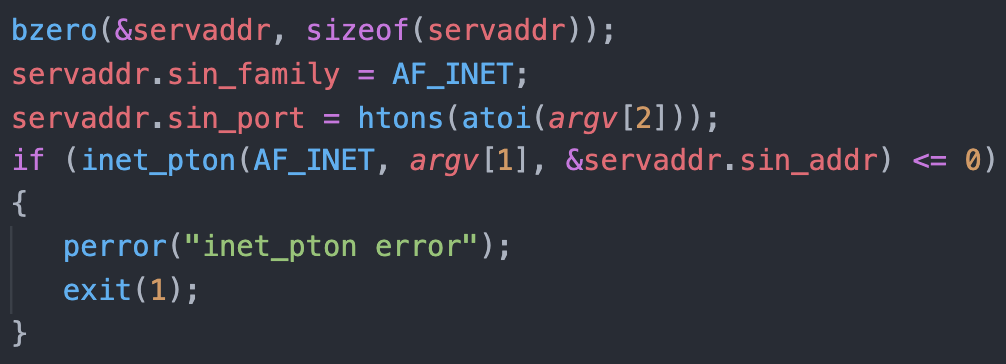
\includegraphics[width=13cm]{images/ex6-cliente-IP.png}
    Além disso, adicionou-se um trecho de código (utilizando a função \textbf{getsockname()}) para mostrar em qual porta local o cliente está conectado.
    \\\\
    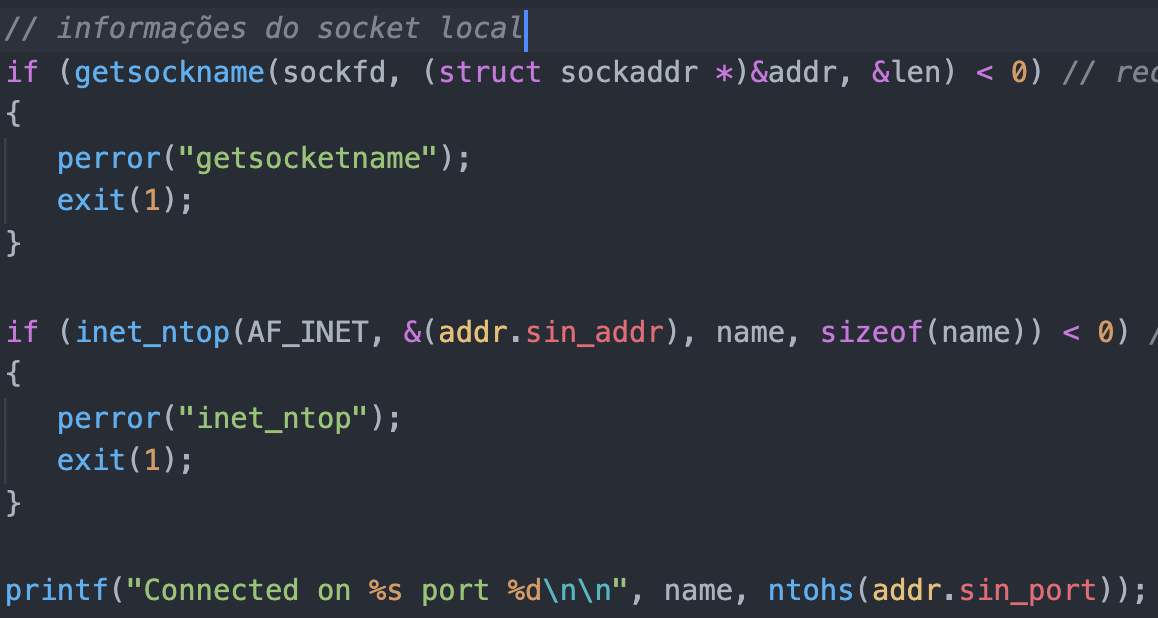
\includegraphics[width=13cm]{images/ex6-cliente-conection.png}
    Servidor:\\\\ 
    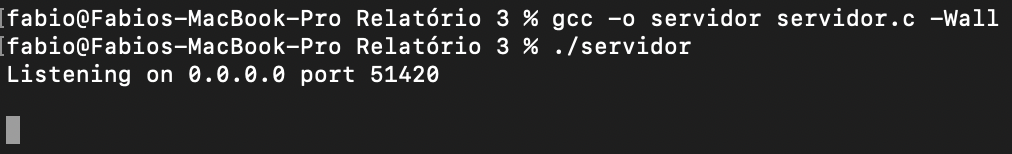
\includegraphics[width=13cm]{images/ex6-servidor-execution.png}
    Cliente:\\\\
    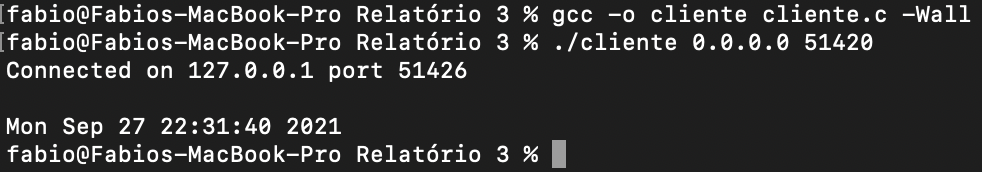
\includegraphics[width=13cm]{images/ex6-cliente-execution.png}

    \item A função \textbf{getpeername()} recupera as informações do endereço do socket do cliente conectado ao servidor (conectado ao socket connfd). Com isso, utilizou-se a função \textbf{inet\_ntop()} para obtermos a representação em string IPv4 do endereço obtido.
    \\\\
    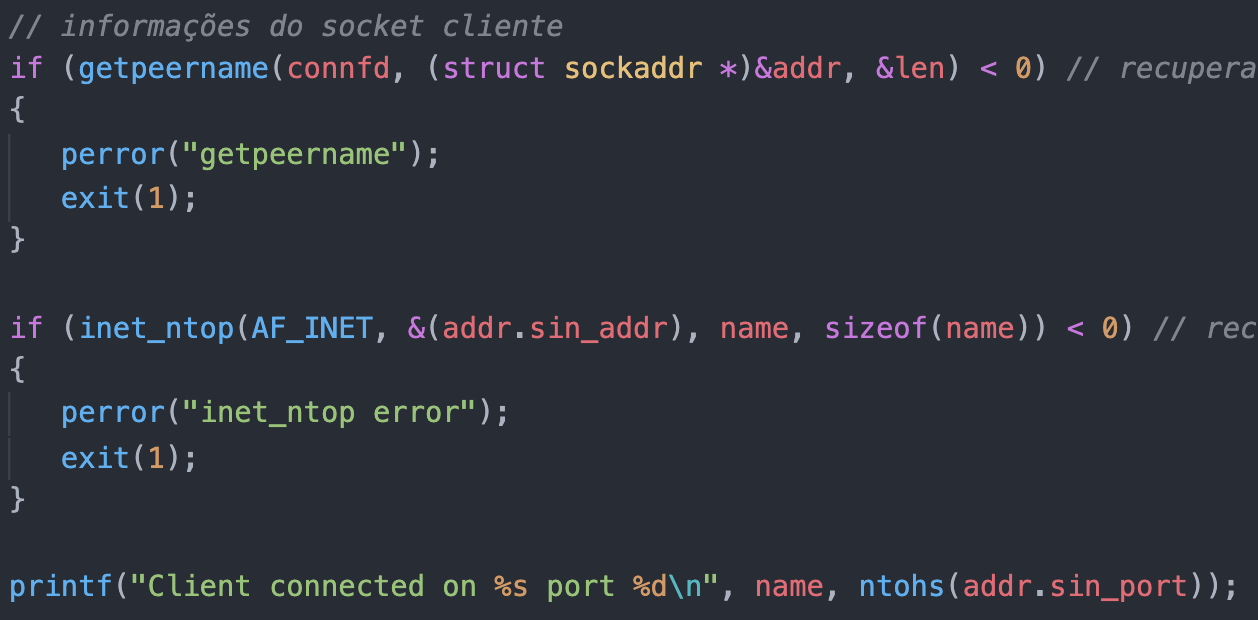
\includegraphics[width=13cm]{images/ex7-servidor.png}\\
    Servidor:\\\\
    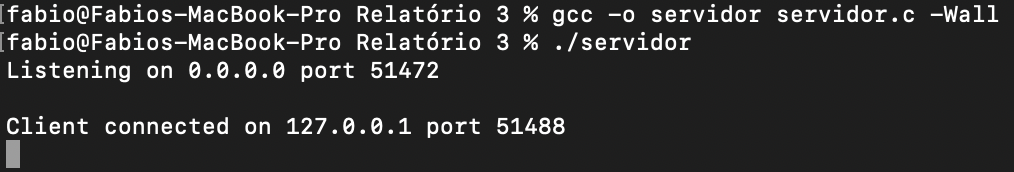
\includegraphics[width=13cm]{images/ex7-execution-servidor.png}\\
    Cliente:\\\\
    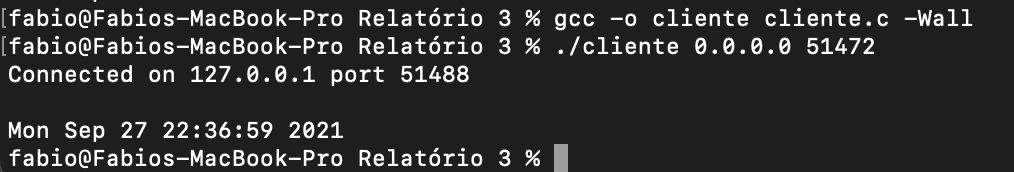
\includegraphics[width=13cm]{images/ex7-execution-cliente.png}
    Nota-se que, nesse exemplo, o servidor está escutando conxões na porta local 51472 e o cliente está conectado na sua porta local 51488.
    
    \item Sim, é possível, uma vez que o comando telnet recebe como parâmetro o endereço IP e a porta em que o servidor está escutando e conecta-se ao mesmo, funcionando da mesma forma que o binário do cliente discutido anteriormente, imprimindo o retorno recebido. A única diferença na execução é que o telnet não imprime qual porta local está conectado com o servidor.
    
    Servidor:\\\\
    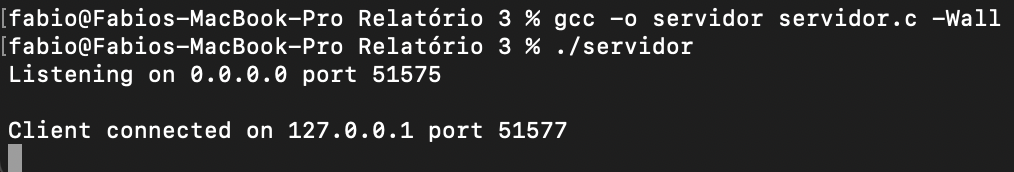
\includegraphics[width=13cm]{images/ex8-servidor.png}\\
    Cliente (telnet):\\\\
    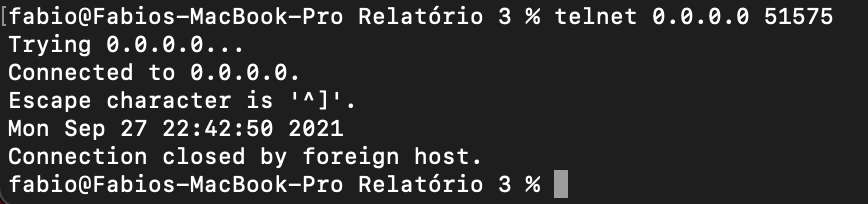
\includegraphics[width=13cm]{images/ex8-cliente.png}
    Nota-se que, nesse exemplo, o servidor está escutando conxões na porta local 51575 e o cliente (telnet) está conectado na sua porta local 51577.
\end{enumerate}

\end{document}
